\documentclass[twoside]{book}

% Packages required by doxygen
\usepackage{fixltx2e}
\usepackage{calc}
\usepackage{doxygen}
\usepackage[export]{adjustbox} % also loads graphicx
\usepackage{graphicx}
\usepackage[utf8]{inputenc}
\usepackage{makeidx}
\usepackage{multicol}
\usepackage{multirow}
\PassOptionsToPackage{warn}{textcomp}
\usepackage{textcomp}
\usepackage[nointegrals]{wasysym}
\usepackage[table]{xcolor}

% Font selection
\usepackage[T1]{fontenc}
\usepackage[scaled=.90]{helvet}
\usepackage{courier}
\usepackage{amssymb}
\usepackage{sectsty}
\renewcommand{\familydefault}{\sfdefault}
\allsectionsfont{%
  \fontseries{bc}\selectfont%
  \color{darkgray}%
}
\renewcommand{\DoxyLabelFont}{%
  \fontseries{bc}\selectfont%
  \color{darkgray}%
}
\newcommand{\+}{\discretionary{\mbox{\scriptsize$\hookleftarrow$}}{}{}}

% Page & text layout
\usepackage{geometry}
\geometry{%
  a4paper,%
  top=2.5cm,%
  bottom=2.5cm,%
  left=2.5cm,%
  right=2.5cm%
}
\tolerance=750
\hfuzz=15pt
\hbadness=750
\setlength{\emergencystretch}{15pt}
\setlength{\parindent}{0cm}
\setlength{\parskip}{3ex plus 2ex minus 2ex}
\makeatletter
\renewcommand{\paragraph}{%
  \@startsection{paragraph}{4}{0ex}{-1.0ex}{1.0ex}{%
    \normalfont\normalsize\bfseries\SS@parafont%
  }%
}
\renewcommand{\subparagraph}{%
  \@startsection{subparagraph}{5}{0ex}{-1.0ex}{1.0ex}{%
    \normalfont\normalsize\bfseries\SS@subparafont%
  }%
}
\makeatother

% Headers & footers
\usepackage{fancyhdr}
\pagestyle{fancyplain}
\fancyhead[LE]{\fancyplain{}{\bfseries\thepage}}
\fancyhead[CE]{\fancyplain{}{}}
\fancyhead[RE]{\fancyplain{}{\bfseries\leftmark}}
\fancyhead[LO]{\fancyplain{}{\bfseries\rightmark}}
\fancyhead[CO]{\fancyplain{}{}}
\fancyhead[RO]{\fancyplain{}{\bfseries\thepage}}
\fancyfoot[LE]{\fancyplain{}{}}
\fancyfoot[CE]{\fancyplain{}{}}
\fancyfoot[RE]{\fancyplain{}{\bfseries\scriptsize Generated by Doxygen }}
\fancyfoot[LO]{\fancyplain{}{\bfseries\scriptsize Generated by Doxygen }}
\fancyfoot[CO]{\fancyplain{}{}}
\fancyfoot[RO]{\fancyplain{}{}}
\renewcommand{\footrulewidth}{0.4pt}
\renewcommand{\chaptermark}[1]{%
  \markboth{#1}{}%
}
\renewcommand{\sectionmark}[1]{%
  \markright{\thesection\ #1}%
}

% Indices & bibliography
\usepackage{natbib}
\usepackage[titles]{tocloft}
\setcounter{tocdepth}{3}
\setcounter{secnumdepth}{5}
\makeindex

% Hyperlinks (required, but should be loaded last)
\usepackage{ifpdf}
\ifpdf
  \usepackage[pdftex,pagebackref=true]{hyperref}
\else
  \usepackage[ps2pdf,pagebackref=true]{hyperref}
\fi
\hypersetup{%
  colorlinks=true,%
  linkcolor=blue,%
  citecolor=blue,%
  unicode%
}

% Custom commands
\newcommand{\clearemptydoublepage}{%
  \newpage{\pagestyle{empty}\cleardoublepage}%
}

\usepackage{caption}
\captionsetup{labelsep=space,justification=centering,font={bf},singlelinecheck=off,skip=4pt,position=top}

%===== C O N T E N T S =====

\begin{document}

% Titlepage & ToC
\hypersetup{pageanchor=false,
             bookmarksnumbered=true,
             pdfencoding=unicode
            }
\pagenumbering{roman}
\begin{titlepage}
\vspace*{7cm}
\begin{center}%
{\Large Robots Algorithm \\[1ex]\large 1.\+0 }\\
\vspace*{1cm}
{\large Generated by Doxygen 1.8.11}\\
\end{center}
\end{titlepage}
\clearemptydoublepage
\tableofcontents
\clearemptydoublepage
\pagenumbering{arabic}
\hypersetup{pageanchor=true}

%--- Begin generated contents ---
\chapter{Hierarchical Index}
\section{Class Hierarchy}
This inheritance list is sorted roughly, but not completely, alphabetically\+:\begin{DoxyCompactList}
\item \contentsline{section}{Application}{\pageref{classApplication}}{}
\begin{DoxyCompactList}
\item \contentsline{section}{Batch\+Application}{\pageref{classBatchApplication}}{}
\item \contentsline{section}{Calibration\+Mode}{\pageref{classCalibrationMode}}{}
\item \contentsline{section}{Interactive\+Application}{\pageref{classInteractiveApplication}}{}
\end{DoxyCompactList}
\item \contentsline{section}{color\+Range}{\pageref{structcolorRange}}{}
\item \contentsline{section}{Detector}{\pageref{classDetector}}{}
\item \contentsline{section}{Extractor}{\pageref{classExtractor}}{}
\item \contentsline{section}{Filter\+Details}{\pageref{structFilterDetails}}{}
\item \contentsline{section}{Filter\+Executor}{\pageref{classFilterExecutor}}{}
\item \contentsline{section}{Parser}{\pageref{classParser}}{}
\item \contentsline{section}{Specification}{\pageref{structSpecification}}{}
\end{DoxyCompactList}

\chapter{Class Index}
\section{Class List}
Here are the classes, structs, unions and interfaces with brief descriptions\+:\begin{DoxyCompactList}
\item\contentsline{section}{\hyperlink{classApplication}{Application} \\*Super class for an application instance. The application can be either the interactive mode, the batchmode and the calibration mode. For each deriving class the pure virtual \hyperlink{classApplication_a7dd8e91a715194dd391be7ae3ecdd985}{run()} function will be implemented and run in the main }{\pageref{classApplication}}{}
\item\contentsline{section}{\hyperlink{classBatchApplication}{Batch\+Application} \\*Instance of an application. The batch application starts the batch mode in the \hyperlink{classBatchApplication_a5338e7513a806b5e751f92d0704d0f8b}{run()} function that stays active until all specifications are handled. The application will display the result for a specification a couple of times (itering as much as specified in frames\+Per\+Spec) before moving to the next specification }{\pageref{classBatchApplication}}{}
\item\contentsline{section}{\hyperlink{classCalibrationMode}{Calibration\+Mode} \\*Calibrationmode is used to calibrate the color ranges. The mode will open up a window with sliders to adjust the color ranges for each color, a window with live frames from the camera and a window that shows the last frame after feature-\/extraction }{\pageref{classCalibrationMode}}{}
\item\contentsline{section}{\hyperlink{structcolorRange}{color\+Range} \\*Struct that contains mapped values for a supported color }{\pageref{structcolorRange}}{}
\item\contentsline{section}{\hyperlink{classDetector}{Detector} \\*The detector class handles all functionality concerning the feature-\/detecting process It will to to recognize pre-\/defined shapes on a binary image (a captured image after feature-\/extracting) }{\pageref{classDetector}}{}
\item\contentsline{section}{\hyperlink{classExtractor}{Extractor} \\*The extractor class filters a raw image untill a simple binary image is left with only the pixels remaining that were in range of the configured color range (minus noise). The feature-\/extraction must always happen before feature-\/detection (read \hyperlink{Detection_8hpp_source}{Detection.\+hpp}) }{\pageref{classExtractor}}{}
\item\contentsline{section}{\hyperlink{structFilterDetails}{Filter\+Details} \\*Struct that contains the details of the filter result for a specific specification }{\pageref{structFilterDetails}}{}
\item\contentsline{section}{\hyperlink{classFilterExecutor}{Filter\+Executor} \\*Filter executor combines the provided functionality by the detection and extraction classes. It will make sure every image is filtered properly and only the shape requested in a specification is marked. When finished it will make sure the result of a specification is showed to the user }{\pageref{classFilterExecutor}}{}
\item\contentsline{section}{\hyperlink{classInteractiveApplication}{Interactive\+Application} \\*Instance of an application. The interactive application starts the interactive mode in the \hyperlink{classInteractiveApplication_ae77593fe90fa4fae53dc8ca84ba1a239}{run()} function that stays active until the user specifies the \textquotesingle{}exit\textquotesingle{} command on the console. The application will display the result for a specification until a new specification is given }{\pageref{classInteractiveApplication}}{}
\item\contentsline{section}{\hyperlink{classParser}{Parser} \\*\hyperlink{classParser}{Parser} contains all functionality to parse batch files and specifications }{\pageref{classParser}}{}
\item\contentsline{section}{\hyperlink{structSpecification}{Specification} \\*Filtering process is based on a specification. This struct describes the attributes a specification has }{\pageref{structSpecification}}{}
\end{DoxyCompactList}

\chapter{Class Documentation}
\hypertarget{classApplication}{}\section{Application Class Reference}
\label{classApplication}\index{Application@{Application}}


the super class for an application instance. The application can be either the interactive mode, the batchmode and the calibration mode. For each deriving class the pure virtual \hyperlink{classApplication_a7dd8e91a715194dd391be7ae3ecdd985}{run()} function will be implemented and run in the main.  




{\ttfamily \#include $<$Application.\+hpp$>$}



Inheritance diagram for Application\+:\nopagebreak
\begin{figure}[H]
\begin{center}
\leavevmode
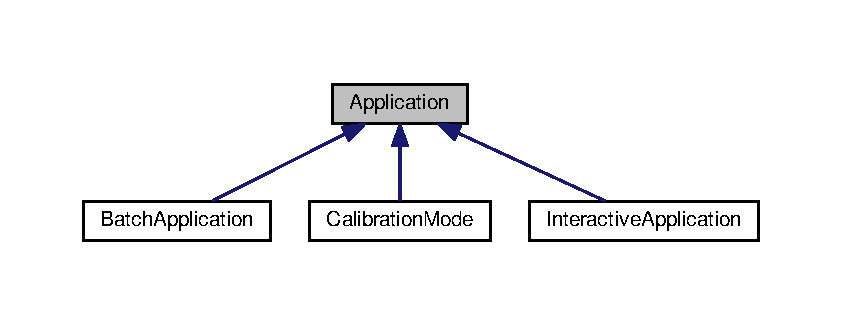
\includegraphics[width=350pt]{classApplication__inherit__graph}
\end{center}
\end{figure}


Collaboration diagram for Application\+:\nopagebreak
\begin{figure}[H]
\begin{center}
\leavevmode
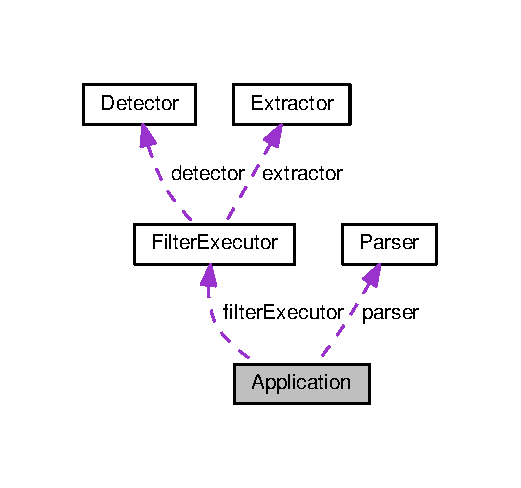
\includegraphics[width=250pt]{classApplication__coll__graph}
\end{center}
\end{figure}
\subsection*{Public Member Functions}
\begin{DoxyCompactItemize}
\item 
\hyperlink{classApplication_a848569c0a80400dba542e8d0cf3726fe}{Application} (const std\+::string \&a\+Name)\hypertarget{classApplication_a848569c0a80400dba542e8d0cf3726fe}{}\label{classApplication_a848569c0a80400dba542e8d0cf3726fe}

\begin{DoxyCompactList}\small\item\em default \hyperlink{classApplication}{Application} constructor \end{DoxyCompactList}\item 
virtual \hyperlink{classApplication_a748bca84fefb9c12661cfaa2f623748d}{$\sim$\+Application} ()\hypertarget{classApplication_a748bca84fefb9c12661cfaa2f623748d}{}\label{classApplication_a748bca84fefb9c12661cfaa2f623748d}

\begin{DoxyCompactList}\small\item\em destructor \end{DoxyCompactList}\item 
virtual void \hyperlink{classApplication_a7dd8e91a715194dd391be7ae3ecdd985}{run} ()=0\hypertarget{classApplication_a7dd8e91a715194dd391be7ae3ecdd985}{}\label{classApplication_a7dd8e91a715194dd391be7ae3ecdd985}

\begin{DoxyCompactList}\small\item\em function that runs a specific instance of an application pure virtual\+: the function gets implemented by its deriving classes \end{DoxyCompactList}\item 
void \hyperlink{classApplication_a05a0e0204f9d319991c0cc5fdc351790}{get\+New\+Frame} ()\hypertarget{classApplication_a05a0e0204f9d319991c0cc5fdc351790}{}\label{classApplication_a05a0e0204f9d319991c0cc5fdc351790}

\begin{DoxyCompactList}\small\item\em Get the New Frame object from the videocapture instance. \end{DoxyCompactList}\end{DoxyCompactItemize}
\subsection*{Protected Attributes}
\begin{DoxyCompactItemize}
\item 
\hyperlink{classParser}{Parser} \hyperlink{classApplication_ad80c2b36d4feb33d203f112d3c890409}{parser}
\item 
std\+::vector$<$ \hyperlink{structSpecification}{Specification} $>$ \hyperlink{classApplication_a041aed976aa156e8265bca7f39c42302}{specifications}
\item 
cv\+::\+Video\+Capture \hyperlink{classApplication_acb0907e73dc0c973aebcf66e34b8034b}{cap}
\item 
cv\+::\+Mat \hyperlink{classApplication_ab33d5d3c05c0077079ed1c9cb66e1775}{frame}
\item 
cv\+::\+Mat \hyperlink{classApplication_a144fb1278bc5e80882b0bd75f077289c}{filtered\+Frame}
\item 
\hyperlink{classFilterExecutor}{Filter\+Executor} \hyperlink{classApplication_a8c2095659954e5914e8be3669264ca61}{filter\+Executor}
\item 
int \hyperlink{classApplication_a181348e18b3debfa1fa2ba936f20967d}{frame\+Refresh\+Rate} = 250
\item 
std\+::string \hyperlink{classApplication_a931b9ffa386916ba1cfd1804823bf51b}{window\+Name}
\item 
bool \hyperlink{classApplication_a09114f3400be3c9907a53be6ec4862af}{active} = true
\end{DoxyCompactItemize}


\subsection{Detailed Description}
the super class for an application instance. The application can be either the interactive mode, the batchmode and the calibration mode. For each deriving class the pure virtual \hyperlink{classApplication_a7dd8e91a715194dd391be7ae3ecdd985}{run()} function will be implemented and run in the main. 

\subsection{Member Data Documentation}
\index{Application@{Application}!active@{active}}
\index{active@{active}!Application@{Application}}
\subsubsection[{\texorpdfstring{active}{active}}]{\setlength{\rightskip}{0pt plus 5cm}bool Application\+::active = true\hspace{0.3cm}{\ttfamily [protected]}}\hypertarget{classApplication_a09114f3400be3c9907a53be6ec4862af}{}\label{classApplication_a09114f3400be3c9907a53be6ec4862af}
Boolean that is true if the application should be active and false if inactive \index{Application@{Application}!cap@{cap}}
\index{cap@{cap}!Application@{Application}}
\subsubsection[{\texorpdfstring{cap}{cap}}]{\setlength{\rightskip}{0pt plus 5cm}cv\+::\+Video\+Capture Application\+::cap\hspace{0.3cm}{\ttfamily [protected]}}\hypertarget{classApplication_acb0907e73dc0c973aebcf66e34b8034b}{}\label{classApplication_acb0907e73dc0c973aebcf66e34b8034b}
The image used is based on a videocapture \index{Application@{Application}!filtered\+Frame@{filtered\+Frame}}
\index{filtered\+Frame@{filtered\+Frame}!Application@{Application}}
\subsubsection[{\texorpdfstring{filtered\+Frame}{filteredFrame}}]{\setlength{\rightskip}{0pt plus 5cm}cv\+::\+Mat Application\+::filtered\+Frame\hspace{0.3cm}{\ttfamily [protected]}}\hypertarget{classApplication_a144fb1278bc5e80882b0bd75f077289c}{}\label{classApplication_a144fb1278bc5e80882b0bd75f077289c}
The filtered frame to be displayed if a specification is given \index{Application@{Application}!filter\+Executor@{filter\+Executor}}
\index{filter\+Executor@{filter\+Executor}!Application@{Application}}
\subsubsection[{\texorpdfstring{filter\+Executor}{filterExecutor}}]{\setlength{\rightskip}{0pt plus 5cm}{\bf Filter\+Executor} Application\+::filter\+Executor\hspace{0.3cm}{\ttfamily [protected]}}\hypertarget{classApplication_a8c2095659954e5914e8be3669264ca61}{}\label{classApplication_a8c2095659954e5914e8be3669264ca61}
The filter executor instance that handles filtering based on specifications \index{Application@{Application}!frame@{frame}}
\index{frame@{frame}!Application@{Application}}
\subsubsection[{\texorpdfstring{frame}{frame}}]{\setlength{\rightskip}{0pt plus 5cm}cv\+::\+Mat Application\+::frame\hspace{0.3cm}{\ttfamily [protected]}}\hypertarget{classApplication_ab33d5d3c05c0077079ed1c9cb66e1775}{}\label{classApplication_ab33d5d3c05c0077079ed1c9cb66e1775}
The last frame captured from the camera \index{Application@{Application}!frame\+Refresh\+Rate@{frame\+Refresh\+Rate}}
\index{frame\+Refresh\+Rate@{frame\+Refresh\+Rate}!Application@{Application}}
\subsubsection[{\texorpdfstring{frame\+Refresh\+Rate}{frameRefreshRate}}]{\setlength{\rightskip}{0pt plus 5cm}int Application\+::frame\+Refresh\+Rate = 250\hspace{0.3cm}{\ttfamily [protected]}}\hypertarget{classApplication_a181348e18b3debfa1fa2ba936f20967d}{}\label{classApplication_a181348e18b3debfa1fa2ba936f20967d}
The time untill the frame refreshes (in milliseconds) \index{Application@{Application}!parser@{parser}}
\index{parser@{parser}!Application@{Application}}
\subsubsection[{\texorpdfstring{parser}{parser}}]{\setlength{\rightskip}{0pt plus 5cm}{\bf Parser} Application\+::parser\hspace{0.3cm}{\ttfamily [protected]}}\hypertarget{classApplication_ad80c2b36d4feb33d203f112d3c890409}{}\label{classApplication_ad80c2b36d4feb33d203f112d3c890409}
Each application has a parser that converts a batchfile or string to a specification \index{Application@{Application}!specifications@{specifications}}
\index{specifications@{specifications}!Application@{Application}}
\subsubsection[{\texorpdfstring{specifications}{specifications}}]{\setlength{\rightskip}{0pt plus 5cm}std\+::vector$<${\bf Specification}$>$ Application\+::specifications\hspace{0.3cm}{\ttfamily [protected]}}\hypertarget{classApplication_a041aed976aa156e8265bca7f39c42302}{}\label{classApplication_a041aed976aa156e8265bca7f39c42302}
An application contains a list with specifications to be executed \index{Application@{Application}!window\+Name@{window\+Name}}
\index{window\+Name@{window\+Name}!Application@{Application}}
\subsubsection[{\texorpdfstring{window\+Name}{windowName}}]{\setlength{\rightskip}{0pt plus 5cm}std\+::string Application\+::window\+Name\hspace{0.3cm}{\ttfamily [protected]}}\hypertarget{classApplication_a931b9ffa386916ba1cfd1804823bf51b}{}\label{classApplication_a931b9ffa386916ba1cfd1804823bf51b}
The name of the cv\+::named\+Window that displays the captured frames 

The documentation for this class was generated from the following files\+:\begin{DoxyCompactItemize}
\item 
src/Application.\+hpp\item 
src/Application.\+cpp\end{DoxyCompactItemize}

\hypertarget{classBatchApplication}{}\section{Batch\+Application Class Reference}
\label{classBatchApplication}\index{Batch\+Application@{Batch\+Application}}


Instance of an application. The batch application starts the batch mode in the \hyperlink{classBatchApplication_a5338e7513a806b5e751f92d0704d0f8b}{run()} function that stays active until all specifications are handled. The application will display the result for a specification a couple of times (itering as much as specified in frames\+Per\+Spec) before moving to the next specification.  




{\ttfamily \#include $<$Batch\+Application.\+hpp$>$}



Inheritance diagram for Batch\+Application\+:\nopagebreak
\begin{figure}[H]
\begin{center}
\leavevmode
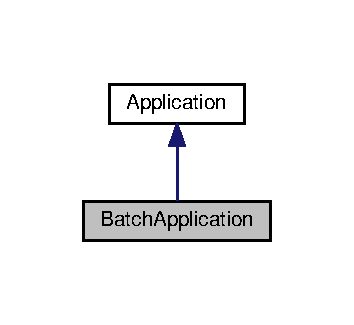
\includegraphics[width=170pt]{classBatchApplication__inherit__graph}
\end{center}
\end{figure}


Collaboration diagram for Batch\+Application\+:\nopagebreak
\begin{figure}[H]
\begin{center}
\leavevmode
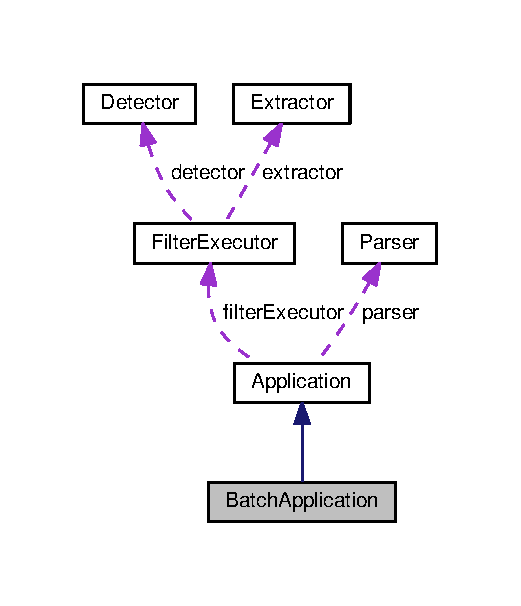
\includegraphics[width=250pt]{classBatchApplication__coll__graph}
\end{center}
\end{figure}
\subsection*{Public Member Functions}
\begin{DoxyCompactItemize}
\item 
\hyperlink{classBatchApplication_ad95d865cf89fe8591f600ffdcf2fd31b}{Batch\+Application} (const std\+::string \&batch\+Config\+Path, const std\+::string \&a\+Name)
\begin{DoxyCompactList}\small\item\em constructor of a batchapplication\+: here the specifications stored in a batch file will be parsed into a list of specifications \end{DoxyCompactList}\item 
virtual \hyperlink{classBatchApplication_a5112919cc14101d58ec2a9f6b884af79}{$\sim$\+Batch\+Application} ()\hypertarget{classBatchApplication_a5112919cc14101d58ec2a9f6b884af79}{}\label{classBatchApplication_a5112919cc14101d58ec2a9f6b884af79}

\begin{DoxyCompactList}\small\item\em destructor of a batchapplication (will be called after the execution of the batch is finished) \end{DoxyCompactList}\item 
void \hyperlink{classBatchApplication_a5338e7513a806b5e751f92d0704d0f8b}{run} ()\hypertarget{classBatchApplication_a5338e7513a806b5e751f92d0704d0f8b}{}\label{classBatchApplication_a5338e7513a806b5e751f92d0704d0f8b}

\begin{DoxyCompactList}\small\item\em function that runs the application\+: overrides the pure virtual run -\/function in \hyperlink{Application_8hpp_source}{Application.\+hpp} \end{DoxyCompactList}\end{DoxyCompactItemize}
\subsection*{Additional Inherited Members}


\subsection{Detailed Description}
Instance of an application. The batch application starts the batch mode in the \hyperlink{classBatchApplication_a5338e7513a806b5e751f92d0704d0f8b}{run()} function that stays active until all specifications are handled. The application will display the result for a specification a couple of times (itering as much as specified in frames\+Per\+Spec) before moving to the next specification. 

\subsection{Constructor \& Destructor Documentation}
\index{Batch\+Application@{Batch\+Application}!Batch\+Application@{Batch\+Application}}
\index{Batch\+Application@{Batch\+Application}!Batch\+Application@{Batch\+Application}}
\subsubsection[{\texorpdfstring{Batch\+Application(const std\+::string \&batch\+Config\+Path, const std\+::string \&a\+Name)}{BatchApplication(const std::string &batchConfigPath, const std::string &aName)}}]{\setlength{\rightskip}{0pt plus 5cm}Batch\+Application\+::\+Batch\+Application (
\begin{DoxyParamCaption}
\item[{const std\+::string \&}]{batch\+Config\+Path, }
\item[{const std\+::string \&}]{a\+Name}
\end{DoxyParamCaption}
)}\hypertarget{classBatchApplication_ad95d865cf89fe8591f600ffdcf2fd31b}{}\label{classBatchApplication_ad95d865cf89fe8591f600ffdcf2fd31b}


constructor of a batchapplication\+: here the specifications stored in a batch file will be parsed into a list of specifications 


\begin{DoxyParams}{Parameters}
{\em batch\+Config\+Path} & the path to the batchfile used in the batchmode \\
\hline
{\em a\+Name} & the name of the window \\
\hline
\end{DoxyParams}


The documentation for this class was generated from the following files\+:\begin{DoxyCompactItemize}
\item 
src/Batch\+Application.\+hpp\item 
src/Batch\+Application.\+cpp\end{DoxyCompactItemize}

\hypertarget{classCalibrationMode}{}\section{Calibration\+Mode Class Reference}
\label{classCalibrationMode}\index{Calibration\+Mode@{Calibration\+Mode}}


the calibrationmode is used to calibrate the color ranges. The mode will open up a window with sliders to adjust the color ranges for each color, a window with live frames from the camera and a window that shows the last frame after feature-\/extraction.  




{\ttfamily \#include $<$Calibration\+Mode.\+hpp$>$}



Inheritance diagram for Calibration\+Mode\+:\nopagebreak
\begin{figure}[H]
\begin{center}
\leavevmode
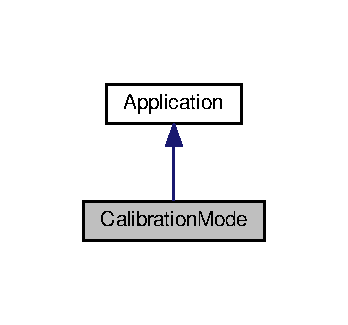
\includegraphics[width=167pt]{classCalibrationMode__inherit__graph}
\end{center}
\end{figure}


Collaboration diagram for Calibration\+Mode\+:\nopagebreak
\begin{figure}[H]
\begin{center}
\leavevmode
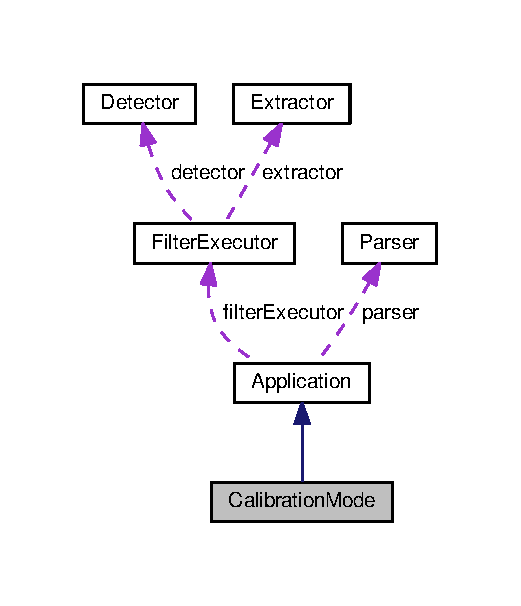
\includegraphics[width=250pt]{classCalibrationMode__coll__graph}
\end{center}
\end{figure}
\subsection*{Public Member Functions}
\begin{DoxyCompactItemize}
\item 
\hyperlink{classCalibrationMode_ac8097b7c6be431d80afad99d3adb73ad}{Calibration\+Mode} (const std\+::string \&a\+Name, const std\+::string \&a\+Calibration\+Window\+Name)
\begin{DoxyCompactList}\small\item\em Construct a new Calibration Mode object. \end{DoxyCompactList}\item 
virtual \hyperlink{classCalibrationMode_a1afa1c5b72412c2b07eb3d508582d366}{$\sim$\+Calibration\+Mode} ()\hypertarget{classCalibrationMode_a1afa1c5b72412c2b07eb3d508582d366}{}\label{classCalibrationMode_a1afa1c5b72412c2b07eb3d508582d366}

\begin{DoxyCompactList}\small\item\em Destroy the Calibration Mode object. \end{DoxyCompactList}\item 
void \hyperlink{classCalibrationMode_a4170e6320aaa744f819340a0064076b9}{run} ()\hypertarget{classCalibrationMode_a4170e6320aaa744f819340a0064076b9}{}\label{classCalibrationMode_a4170e6320aaa744f819340a0064076b9}

\begin{DoxyCompactList}\small\item\em function that runs the application\+: overrides the pure virtual run -\/function in \hyperlink{Application_8hpp_source}{Application.\+hpp} \end{DoxyCompactList}\item 
void \hyperlink{classCalibrationMode_ad3c3850c2ed080d299f6e4e5a3e1cd87}{update\+Set\+Range} ()\hypertarget{classCalibrationMode_ad3c3850c2ed080d299f6e4e5a3e1cd87}{}\label{classCalibrationMode_ad3c3850c2ed080d299f6e4e5a3e1cd87}

\begin{DoxyCompactList}\small\item\em function that updates the ranges set on the slider to the map \end{DoxyCompactList}\end{DoxyCompactItemize}
\subsection*{Static Public Member Functions}
\begin{DoxyCompactItemize}
\item 
static void \hyperlink{classCalibrationMode_a9b78a49f8a37355e1563d5f4f52b0136}{calibrate} (int v, void $\ast$ptr)
\begin{DoxyCompactList}\small\item\em static function used as callback by the trackbar sliders from open\+CV \end{DoxyCompactList}\end{DoxyCompactItemize}
\subsection*{Additional Inherited Members}


\subsection{Detailed Description}
the calibrationmode is used to calibrate the color ranges. The mode will open up a window with sliders to adjust the color ranges for each color, a window with live frames from the camera and a window that shows the last frame after feature-\/extraction. 

\subsection{Constructor \& Destructor Documentation}
\index{Calibration\+Mode@{Calibration\+Mode}!Calibration\+Mode@{Calibration\+Mode}}
\index{Calibration\+Mode@{Calibration\+Mode}!Calibration\+Mode@{Calibration\+Mode}}
\subsubsection[{\texorpdfstring{Calibration\+Mode(const std\+::string \&a\+Name, const std\+::string \&a\+Calibration\+Window\+Name)}{CalibrationMode(const std::string &aName, const std::string &aCalibrationWindowName)}}]{\setlength{\rightskip}{0pt plus 5cm}Calibration\+Mode\+::\+Calibration\+Mode (
\begin{DoxyParamCaption}
\item[{const std\+::string \&}]{a\+Name, }
\item[{const std\+::string \&}]{a\+Calibration\+Window\+Name}
\end{DoxyParamCaption}
)}\hypertarget{classCalibrationMode_ac8097b7c6be431d80afad99d3adb73ad}{}\label{classCalibrationMode_ac8097b7c6be431d80afad99d3adb73ad}


Construct a new Calibration Mode object. 


\begin{DoxyParams}{Parameters}
{\em a\+Name} & the name of the camera window \\
\hline
{\em a\+Calibration\+Window\+Name} & \\
\hline
\end{DoxyParams}


\subsection{Member Function Documentation}
\index{Calibration\+Mode@{Calibration\+Mode}!calibrate@{calibrate}}
\index{calibrate@{calibrate}!Calibration\+Mode@{Calibration\+Mode}}
\subsubsection[{\texorpdfstring{calibrate(int v, void $\ast$ptr)}{calibrate(int v, void *ptr)}}]{\setlength{\rightskip}{0pt plus 5cm}static void Calibration\+Mode\+::calibrate (
\begin{DoxyParamCaption}
\item[{int}]{v, }
\item[{void $\ast$}]{ptr}
\end{DoxyParamCaption}
)\hspace{0.3cm}{\ttfamily [inline]}, {\ttfamily [static]}}\hypertarget{classCalibrationMode_a9b78a49f8a37355e1563d5f4f52b0136}{}\label{classCalibrationMode_a9b78a49f8a37355e1563d5f4f52b0136}


static function used as callback by the trackbar sliders from open\+CV 


\begin{DoxyParams}{Parameters}
{\em v} & \\
\hline
{\em ptr} & this instance of the object instance \\
\hline
\end{DoxyParams}


The documentation for this class was generated from the following files\+:\begin{DoxyCompactItemize}
\item 
src/Calibration\+Mode.\+hpp\item 
src/Calibration\+Mode.\+cpp\end{DoxyCompactItemize}

\hypertarget{structcolorRange}{}\section{color\+Range Struct Reference}
\label{structcolorRange}\index{color\+Range@{color\+Range}}


Struct that contains mapped values for a supported color.  




{\ttfamily \#include $<$Specification\+Config.\+hpp$>$}

\subsection*{Public Attributes}
\begin{DoxyCompactItemize}
\item 
int \hyperlink{structcolorRange_a9679488c6339699971dd203817216c0c}{min\+Hue}
\item 
int \hyperlink{structcolorRange_a08f7a79d3fe6da4ce3dd62ac710cb8b9}{max\+Hue}
\item 
int \hyperlink{structcolorRange_a98acafa32db912103eeb515b6f8308a0}{min\+Saturation}
\item 
int \hyperlink{structcolorRange_abf29d6b695efd30da709e39b4c94b638}{max\+Saturation}
\item 
int \hyperlink{structcolorRange_a51150443fec527eab104fc39d6811bd8}{min\+Value}
\item 
int \hyperlink{structcolorRange_a1653821b47f0de18315b0d7f3bc54c13}{max\+Value}
\end{DoxyCompactItemize}


\subsection{Detailed Description}
Struct that contains mapped values for a supported color. 

\subsection{Member Data Documentation}
\index{color\+Range@{color\+Range}!max\+Hue@{max\+Hue}}
\index{max\+Hue@{max\+Hue}!color\+Range@{color\+Range}}
\subsubsection[{\texorpdfstring{max\+Hue}{maxHue}}]{\setlength{\rightskip}{0pt plus 5cm}int color\+Range\+::max\+Hue}\hypertarget{structcolorRange_a08f7a79d3fe6da4ce3dd62ac710cb8b9}{}\label{structcolorRange_a08f7a79d3fe6da4ce3dd62ac710cb8b9}
Maximum hue (0-\/179) for a specific color \index{color\+Range@{color\+Range}!max\+Saturation@{max\+Saturation}}
\index{max\+Saturation@{max\+Saturation}!color\+Range@{color\+Range}}
\subsubsection[{\texorpdfstring{max\+Saturation}{maxSaturation}}]{\setlength{\rightskip}{0pt plus 5cm}int color\+Range\+::max\+Saturation}\hypertarget{structcolorRange_abf29d6b695efd30da709e39b4c94b638}{}\label{structcolorRange_abf29d6b695efd30da709e39b4c94b638}
Maximum saturation (0-\/255) for a specific color \index{color\+Range@{color\+Range}!max\+Value@{max\+Value}}
\index{max\+Value@{max\+Value}!color\+Range@{color\+Range}}
\subsubsection[{\texorpdfstring{max\+Value}{maxValue}}]{\setlength{\rightskip}{0pt plus 5cm}int color\+Range\+::max\+Value}\hypertarget{structcolorRange_a1653821b47f0de18315b0d7f3bc54c13}{}\label{structcolorRange_a1653821b47f0de18315b0d7f3bc54c13}
Maximum value (0-\/255) for a specific color \index{color\+Range@{color\+Range}!min\+Hue@{min\+Hue}}
\index{min\+Hue@{min\+Hue}!color\+Range@{color\+Range}}
\subsubsection[{\texorpdfstring{min\+Hue}{minHue}}]{\setlength{\rightskip}{0pt plus 5cm}int color\+Range\+::min\+Hue}\hypertarget{structcolorRange_a9679488c6339699971dd203817216c0c}{}\label{structcolorRange_a9679488c6339699971dd203817216c0c}
Minimum hue (0-\/179) for a specific color \index{color\+Range@{color\+Range}!min\+Saturation@{min\+Saturation}}
\index{min\+Saturation@{min\+Saturation}!color\+Range@{color\+Range}}
\subsubsection[{\texorpdfstring{min\+Saturation}{minSaturation}}]{\setlength{\rightskip}{0pt plus 5cm}int color\+Range\+::min\+Saturation}\hypertarget{structcolorRange_a98acafa32db912103eeb515b6f8308a0}{}\label{structcolorRange_a98acafa32db912103eeb515b6f8308a0}
Minimum saturation (0-\/255) for a specific color \index{color\+Range@{color\+Range}!min\+Value@{min\+Value}}
\index{min\+Value@{min\+Value}!color\+Range@{color\+Range}}
\subsubsection[{\texorpdfstring{min\+Value}{minValue}}]{\setlength{\rightskip}{0pt plus 5cm}int color\+Range\+::min\+Value}\hypertarget{structcolorRange_a51150443fec527eab104fc39d6811bd8}{}\label{structcolorRange_a51150443fec527eab104fc39d6811bd8}
Minimum value (0-\/255) for a specific color 

The documentation for this struct was generated from the following file\+:\begin{DoxyCompactItemize}
\item 
src/Specification\+Config.\+hpp\end{DoxyCompactItemize}

\hypertarget{classDetector}{}\section{Detector Class Reference}
\label{classDetector}\index{Detector@{Detector}}


The detector class handles all functionality concerning the feature-\/detecting process It will to to recognize pre-\/defined shapes on a binary image (a captured image after feature-\/extracting)  




{\ttfamily \#include $<$Detection.\+hpp$>$}

\subsection*{Public Member Functions}
\begin{DoxyCompactItemize}
\item 
\hyperlink{classDetector_aa43b3d7bbd4b225855b4bcc93f70b225}{Detector} ()\hypertarget{classDetector_aa43b3d7bbd4b225855b4bcc93f70b225}{}\label{classDetector_aa43b3d7bbd4b225855b4bcc93f70b225}

\begin{DoxyCompactList}\small\item\em Construct a new \hyperlink{classDetector}{Detector} object. \end{DoxyCompactList}\item 
virtual \hyperlink{classDetector_ae16b7bf62f39cb287927d56ca17663d7}{$\sim$\+Detector} ()\hypertarget{classDetector_ae16b7bf62f39cb287927d56ca17663d7}{}\label{classDetector_ae16b7bf62f39cb287927d56ca17663d7}

\begin{DoxyCompactList}\small\item\em Destroy the \hyperlink{classDetector}{Detector} object. \end{DoxyCompactList}\item 
double \hyperlink{classDetector_a8357eef6f384fe126ebf511e21f592f4}{cosine\+Law} (const double a, const double b, const double c) const 
\begin{DoxyCompactList}\small\item\em implementation of the cosine law (see inline comments in .cpp file) \end{DoxyCompactList}\item 
bool \hyperlink{classDetector_a646cf1117d58014c700b18fe21318d1b}{check\+If\+Square} (const std\+::vector$<$ std\+::vector$<$ cv\+::\+Point $>$$>$ \&contours, int index, \hyperlink{structFilterDetails}{Filter\+Details} \&filter\+Details) const 
\begin{DoxyCompactList}\small\item\em function that checks if a shape is a square based on surface, width and height \end{DoxyCompactList}\item 
bool \hyperlink{classDetector_a11701ce9ed01a8cbc0e12e3f7d30fc59}{check\+If\+Triangle} (const std\+::vector$<$ std\+::vector$<$ cv\+::\+Point $>$$>$ \&contours, int index, \hyperlink{structFilterDetails}{Filter\+Details} \&filter\+Details) const 
\begin{DoxyCompactList}\small\item\em function that checks if a shape is a triangle based on surface and total of the three angles \end{DoxyCompactList}\item 
bool \hyperlink{classDetector_a04bb1c8b13c2902e322bdb5533dc24d4}{check\+If\+Rect} (const std\+::vector$<$ std\+::vector$<$ cv\+::\+Point $>$$>$ \&contours, int index, \hyperlink{structFilterDetails}{Filter\+Details} \&filter\+Details) const 
\begin{DoxyCompactList}\small\item\em function that checks if a shape is a rectangle (a square is also a rectangle) \end{DoxyCompactList}\item 
bool \hyperlink{classDetector_a93e674f8779b04318ec20e14b9f29fa3}{check\+If\+Circle} (const std\+::vector$<$ std\+::vector$<$ cv\+::\+Point $>$$>$ \&contours, int index, \hyperlink{structFilterDetails}{Filter\+Details} \&filter\+Details) const 
\begin{DoxyCompactList}\small\item\em function that checks if a shape is a circle \end{DoxyCompactList}\item 
bool \hyperlink{classDetector_aded5bb3b41a972a3bc97698c07cece6b}{check\+If\+Half\+Circle} (const std\+::vector$<$ std\+::vector$<$ cv\+::\+Point $>$$>$ \&contours, int index, \hyperlink{structFilterDetails}{Filter\+Details} \&filter\+Details) const 
\begin{DoxyCompactList}\small\item\em function that checks if a shape is half a circle \end{DoxyCompactList}\item 
std\+::optional$<$ supported\+Shape $>$ \hyperlink{classDetector_a4e9d90d69c0400d48a6b8a3b35b91d77}{detect\+Shape} (const std\+::vector$<$ cv\+::\+Point $>$ \&contour) const 
\begin{DoxyCompactList}\small\item\em function that detects a shape if it matches (enough) with a reference shape \end{DoxyCompactList}\end{DoxyCompactItemize}


\subsection{Detailed Description}
The detector class handles all functionality concerning the feature-\/detecting process It will to to recognize pre-\/defined shapes on a binary image (a captured image after feature-\/extracting) 

\subsection{Member Function Documentation}
\index{Detector@{Detector}!check\+If\+Circle@{check\+If\+Circle}}
\index{check\+If\+Circle@{check\+If\+Circle}!Detector@{Detector}}
\subsubsection[{\texorpdfstring{check\+If\+Circle(const std\+::vector$<$ std\+::vector$<$ cv\+::\+Point $>$$>$ \&contours, int index, Filter\+Details \&filter\+Details) const }{checkIfCircle(const std::vector< std::vector< cv::Point >> &contours, int index, FilterDetails &filterDetails) const }}]{\setlength{\rightskip}{0pt plus 5cm}bool Detector\+::check\+If\+Circle (
\begin{DoxyParamCaption}
\item[{const std\+::vector$<$ std\+::vector$<$ cv\+::\+Point $>$$>$ \&}]{contours, }
\item[{int}]{index, }
\item[{{\bf Filter\+Details} \&}]{filter\+Details}
\end{DoxyParamCaption}
) const}\hypertarget{classDetector_a93e674f8779b04318ec20e14b9f29fa3}{}\label{classDetector_a93e674f8779b04318ec20e14b9f29fa3}


function that checks if a shape is a circle 


\begin{DoxyParams}{Parameters}
{\em contours} & the contours detected \\
\hline
{\em index} & the index of the contour to be detected \\
\hline
{\em filter\+Details} & the result (details) of the detection for a specific set of contours \\
\hline
\end{DoxyParams}
\begin{DoxyReturn}{Returns}
true if the contours matches with the definition of a square 

false if the contours don\textquotesingle{}t match with the definition of a circle
\end{DoxyReturn}
A circle is a shape where the surface of the shape is equal to π $\ast$ r2 \&\& Each line from the center to the border has the same length \index{Detector@{Detector}!check\+If\+Half\+Circle@{check\+If\+Half\+Circle}}
\index{check\+If\+Half\+Circle@{check\+If\+Half\+Circle}!Detector@{Detector}}
\subsubsection[{\texorpdfstring{check\+If\+Half\+Circle(const std\+::vector$<$ std\+::vector$<$ cv\+::\+Point $>$$>$ \&contours, int index, Filter\+Details \&filter\+Details) const }{checkIfHalfCircle(const std::vector< std::vector< cv::Point >> &contours, int index, FilterDetails &filterDetails) const }}]{\setlength{\rightskip}{0pt plus 5cm}bool Detector\+::check\+If\+Half\+Circle (
\begin{DoxyParamCaption}
\item[{const std\+::vector$<$ std\+::vector$<$ cv\+::\+Point $>$$>$ \&}]{contours, }
\item[{int}]{index, }
\item[{{\bf Filter\+Details} \&}]{filter\+Details}
\end{DoxyParamCaption}
) const}\hypertarget{classDetector_aded5bb3b41a972a3bc97698c07cece6b}{}\label{classDetector_aded5bb3b41a972a3bc97698c07cece6b}


function that checks if a shape is half a circle 


\begin{DoxyParams}{Parameters}
{\em contours} & the contours detected \\
\hline
{\em index} & the index of the contour to be detected \\
\hline
{\em filter\+Details} & the result (details) of the detection for a specific set of contours \\
\hline
\end{DoxyParams}
\begin{DoxyReturn}{Returns}
true if the contours matches with the definition of a square 

false if the contours don\textquotesingle{}t match with the definition of half a circle 
\end{DoxyReturn}
\index{Detector@{Detector}!check\+If\+Rect@{check\+If\+Rect}}
\index{check\+If\+Rect@{check\+If\+Rect}!Detector@{Detector}}
\subsubsection[{\texorpdfstring{check\+If\+Rect(const std\+::vector$<$ std\+::vector$<$ cv\+::\+Point $>$$>$ \&contours, int index, Filter\+Details \&filter\+Details) const }{checkIfRect(const std::vector< std::vector< cv::Point >> &contours, int index, FilterDetails &filterDetails) const }}]{\setlength{\rightskip}{0pt plus 5cm}bool Detector\+::check\+If\+Rect (
\begin{DoxyParamCaption}
\item[{const std\+::vector$<$ std\+::vector$<$ cv\+::\+Point $>$$>$ \&}]{contours, }
\item[{int}]{index, }
\item[{{\bf Filter\+Details} \&}]{filter\+Details}
\end{DoxyParamCaption}
) const}\hypertarget{classDetector_a04bb1c8b13c2902e322bdb5533dc24d4}{}\label{classDetector_a04bb1c8b13c2902e322bdb5533dc24d4}


function that checks if a shape is a rectangle (a square is also a rectangle) 


\begin{DoxyParams}{Parameters}
{\em contours} & the contours detected \\
\hline
{\em index} & the index of the contour to be detected \\
\hline
{\em filter\+Details} & the result (details) of the detection for a specific set of contours \\
\hline
\end{DoxyParams}
\begin{DoxyReturn}{Returns}
true if the contours matches with the definition of a square 

false if the contours don\textquotesingle{}t match with the definition of a rectangle 
\end{DoxyReturn}
\index{Detector@{Detector}!check\+If\+Square@{check\+If\+Square}}
\index{check\+If\+Square@{check\+If\+Square}!Detector@{Detector}}
\subsubsection[{\texorpdfstring{check\+If\+Square(const std\+::vector$<$ std\+::vector$<$ cv\+::\+Point $>$$>$ \&contours, int index, Filter\+Details \&filter\+Details) const }{checkIfSquare(const std::vector< std::vector< cv::Point >> &contours, int index, FilterDetails &filterDetails) const }}]{\setlength{\rightskip}{0pt plus 5cm}bool Detector\+::check\+If\+Square (
\begin{DoxyParamCaption}
\item[{const std\+::vector$<$ std\+::vector$<$ cv\+::\+Point $>$$>$ \&}]{contours, }
\item[{int}]{index, }
\item[{{\bf Filter\+Details} \&}]{filter\+Details}
\end{DoxyParamCaption}
) const}\hypertarget{classDetector_a646cf1117d58014c700b18fe21318d1b}{}\label{classDetector_a646cf1117d58014c700b18fe21318d1b}


function that checks if a shape is a square based on surface, width and height 


\begin{DoxyParams}{Parameters}
{\em contours} & the contours detected \\
\hline
{\em index} & the index of the contour to be detected \\
\hline
{\em filter\+Details} & the result (details) of the detection for a specific set of contours \\
\hline
\end{DoxyParams}
\begin{DoxyReturn}{Returns}
true if the contours matches with the definition of a square 

false if the contours don\textquotesingle{}t match with the definition of a square 
\end{DoxyReturn}
Factor determines how close the detected shape should be to a square to be treated like a square

Any side is $>$ base side divided by the factor\+: return false

Else\+: the shape is (close enough to) a square\+: return true \index{Detector@{Detector}!check\+If\+Triangle@{check\+If\+Triangle}}
\index{check\+If\+Triangle@{check\+If\+Triangle}!Detector@{Detector}}
\subsubsection[{\texorpdfstring{check\+If\+Triangle(const std\+::vector$<$ std\+::vector$<$ cv\+::\+Point $>$$>$ \&contours, int index, Filter\+Details \&filter\+Details) const }{checkIfTriangle(const std::vector< std::vector< cv::Point >> &contours, int index, FilterDetails &filterDetails) const }}]{\setlength{\rightskip}{0pt plus 5cm}bool Detector\+::check\+If\+Triangle (
\begin{DoxyParamCaption}
\item[{const std\+::vector$<$ std\+::vector$<$ cv\+::\+Point $>$$>$ \&}]{contours, }
\item[{int}]{index, }
\item[{{\bf Filter\+Details} \&}]{filter\+Details}
\end{DoxyParamCaption}
) const}\hypertarget{classDetector_a11701ce9ed01a8cbc0e12e3f7d30fc59}{}\label{classDetector_a11701ce9ed01a8cbc0e12e3f7d30fc59}


function that checks if a shape is a triangle based on surface and total of the three angles 


\begin{DoxyParams}{Parameters}
{\em contours} & the contours detected \\
\hline
{\em index} & the index of the contour to be detected \\
\hline
{\em filter\+Details} & the result (details) of the detection for a specific set of contours \\
\hline
\end{DoxyParams}
\begin{DoxyReturn}{Returns}
true if the contours matches with the definition of a square 

false if the contours don\textquotesingle{}t match with the definition of a triangle
\end{DoxyReturn}
A triangle is a closed shape with 3 angles where the sum of 3 angles is (almost) equal to 180° The triangle has been allowed a deviation of 1.\+0° relative to 180°

If the total of the three corners dont add up to +/-\/ 180° the shape is not a triangle \index{Detector@{Detector}!cosine\+Law@{cosine\+Law}}
\index{cosine\+Law@{cosine\+Law}!Detector@{Detector}}
\subsubsection[{\texorpdfstring{cosine\+Law(const double a, const double b, const double c) const }{cosineLaw(const double a, const double b, const double c) const }}]{\setlength{\rightskip}{0pt plus 5cm}double Detector\+::cosine\+Law (
\begin{DoxyParamCaption}
\item[{const double}]{a, }
\item[{const double}]{b, }
\item[{const double}]{c}
\end{DoxyParamCaption}
) const}\hypertarget{classDetector_a8357eef6f384fe126ebf511e21f592f4}{}\label{classDetector_a8357eef6f384fe126ebf511e21f592f4}


implementation of the cosine law (see inline comments in .cpp file) 


\begin{DoxyParams}{Parameters}
{\em a} & first width \\
\hline
{\em b} & second width \\
\hline
{\em c} & third width \\
\hline
\end{DoxyParams}
\begin{DoxyReturn}{Returns}
double the angle
\end{DoxyReturn}
Implementation based on\+: \href{https://en.wikipedia.org/wiki/Law_of_cosines}{\tt https\+://en.\+wikipedia.\+org/wiki/\+Law\+\_\+of\+\_\+cosines} C++ implementation of\+: \textquotesingle{}a² = b² + c² -\/2bc $\ast$ cos(\+A)\textquotesingle{} \index{Detector@{Detector}!detect\+Shape@{detect\+Shape}}
\index{detect\+Shape@{detect\+Shape}!Detector@{Detector}}
\subsubsection[{\texorpdfstring{detect\+Shape(const std\+::vector$<$ cv\+::\+Point $>$ \&contour) const }{detectShape(const std::vector< cv::Point > &contour) const }}]{\setlength{\rightskip}{0pt plus 5cm}std\+::optional$<$ supported\+Shape $>$ Detector\+::detect\+Shape (
\begin{DoxyParamCaption}
\item[{const std\+::vector$<$ cv\+::\+Point $>$ \&}]{contour}
\end{DoxyParamCaption}
) const}\hypertarget{classDetector_a4e9d90d69c0400d48a6b8a3b35b91d77}{}\label{classDetector_a4e9d90d69c0400d48a6b8a3b35b91d77}


function that detects a shape if it matches (enough) with a reference shape 


\begin{DoxyParams}{Parameters}
{\em contour} & the contour to be detected \\
\hline
\end{DoxyParams}
\begin{DoxyReturn}{Returns}
std\+::optional$<$supported\+Shape$>$ nullopt if the shape didn\textquotesingle{}t match enough with any reference shape, else the shape it matches the most with 
\end{DoxyReturn}


The documentation for this class was generated from the following files\+:\begin{DoxyCompactItemize}
\item 
src/Detection.\+hpp\item 
src/Detection.\+cpp\end{DoxyCompactItemize}

\hypertarget{classExtractor}{}\section{Extractor Class Reference}
\label{classExtractor}\index{Extractor@{Extractor}}


The extractor class filters a raw image untill a simple binary image is left with only the pixels remaining that were in range of the configured color range (minus noise). The feature-\/extraction must always happen before feature-\/detection (read \hyperlink{Detection_8hpp_source}{Detection.\+hpp}).  




{\ttfamily \#include $<$Extraction.\+hpp$>$}

\subsection*{Public Member Functions}
\begin{DoxyCompactItemize}
\item 
\hyperlink{classExtractor_a2726e6a94c51c2b2dbc518199d054103}{Extractor} ()\hypertarget{classExtractor_a2726e6a94c51c2b2dbc518199d054103}{}\label{classExtractor_a2726e6a94c51c2b2dbc518199d054103}

\begin{DoxyCompactList}\small\item\em Construct a new \hyperlink{classExtractor}{Extractor} object. \end{DoxyCompactList}\item 
virtual \hyperlink{classExtractor_a0da249c590c92ed0714e8bd69ac236f4}{$\sim$\+Extractor} ()\hypertarget{classExtractor_a0da249c590c92ed0714e8bd69ac236f4}{}\label{classExtractor_a0da249c590c92ed0714e8bd69ac236f4}

\begin{DoxyCompactList}\small\item\em Destroy the \hyperlink{classExtractor}{Extractor} object. \end{DoxyCompactList}\item 
cv\+::\+Mat \hyperlink{classExtractor_a89c360e740a37c38e6ef23185f5cb862}{extract} (const cv\+::\+Mat \&original, const supported\+Color \&color) const 
\begin{DoxyCompactList}\small\item\em function that extracts the image based on a selected color All pixels that are not in range of the color-\/range and noise will be removed \end{DoxyCompactList}\item 
std\+::map$<$ supported\+Color, \hyperlink{structcolorRange}{color\+Range} $>$ \hyperlink{classExtractor_ab48284118c37aff704e714f9a6da1331}{mapped\+Color\+Ranges\+Map\+From\+File} () const 
\begin{DoxyCompactList}\small\item\em function that parses a config file with color ranges to a map \end{DoxyCompactList}\item 
void \hyperlink{classExtractor_adfd9ce2b8cee262883ee94a5e27e1d69}{mapped\+Color\+Ranges\+Map\+To\+File} (const std\+::map$<$ supported\+Color, \hyperlink{structcolorRange}{color\+Range} $>$ \&a\+Mapped\+Color\+Ranges\+Map)
\begin{DoxyCompactList}\small\item\em function that parses a map with color ranges to a config file \end{DoxyCompactList}\end{DoxyCompactItemize}


\subsection{Detailed Description}
The extractor class filters a raw image untill a simple binary image is left with only the pixels remaining that were in range of the configured color range (minus noise). The feature-\/extraction must always happen before feature-\/detection (read \hyperlink{Detection_8hpp_source}{Detection.\+hpp}). 

\subsection{Member Function Documentation}
\index{Extractor@{Extractor}!extract@{extract}}
\index{extract@{extract}!Extractor@{Extractor}}
\subsubsection[{\texorpdfstring{extract(const cv\+::\+Mat \&original, const supported\+Color \&color) const }{extract(const cv::Mat &original, const supportedColor &color) const }}]{\setlength{\rightskip}{0pt plus 5cm}cv\+::\+Mat Extractor\+::extract (
\begin{DoxyParamCaption}
\item[{const cv\+::\+Mat \&}]{original, }
\item[{const supported\+Color \&}]{color}
\end{DoxyParamCaption}
) const}\hypertarget{classExtractor_a89c360e740a37c38e6ef23185f5cb862}{}\label{classExtractor_a89c360e740a37c38e6ef23185f5cb862}


function that extracts the image based on a selected color All pixels that are not in range of the color-\/range and noise will be removed 


\begin{DoxyParams}{Parameters}
{\em original} & the raw (not converted) image object \\
\hline
{\em color} & the requested color \\
\hline
\end{DoxyParams}
\begin{DoxyReturn}{Returns}
cv\+::\+Mat the extracted image (with only the relevant pixels remaining) 
\end{DoxyReturn}
\index{Extractor@{Extractor}!mapped\+Color\+Ranges\+Map\+From\+File@{mapped\+Color\+Ranges\+Map\+From\+File}}
\index{mapped\+Color\+Ranges\+Map\+From\+File@{mapped\+Color\+Ranges\+Map\+From\+File}!Extractor@{Extractor}}
\subsubsection[{\texorpdfstring{mapped\+Color\+Ranges\+Map\+From\+File() const }{mappedColorRangesMapFromFile() const }}]{\setlength{\rightskip}{0pt plus 5cm}std\+::map$<$ supported\+Color, {\bf color\+Range} $>$ Extractor\+::mapped\+Color\+Ranges\+Map\+From\+File (
\begin{DoxyParamCaption}
{}
\end{DoxyParamCaption}
) const}\hypertarget{classExtractor_ab48284118c37aff704e714f9a6da1331}{}\label{classExtractor_ab48284118c37aff704e714f9a6da1331}


function that parses a config file with color ranges to a map 

\begin{DoxyReturn}{Returns}
std\+::map$<$supported\+Color, color\+Range$>$ the converted ranges stored in a map 
\end{DoxyReturn}
\index{Extractor@{Extractor}!mapped\+Color\+Ranges\+Map\+To\+File@{mapped\+Color\+Ranges\+Map\+To\+File}}
\index{mapped\+Color\+Ranges\+Map\+To\+File@{mapped\+Color\+Ranges\+Map\+To\+File}!Extractor@{Extractor}}
\subsubsection[{\texorpdfstring{mapped\+Color\+Ranges\+Map\+To\+File(const std\+::map$<$ supported\+Color, color\+Range $>$ \&a\+Mapped\+Color\+Ranges\+Map)}{mappedColorRangesMapToFile(const std::map< supportedColor, colorRange > &aMappedColorRangesMap)}}]{\setlength{\rightskip}{0pt plus 5cm}void Extractor\+::mapped\+Color\+Ranges\+Map\+To\+File (
\begin{DoxyParamCaption}
\item[{const std\+::map$<$ supported\+Color, {\bf color\+Range} $>$ \&}]{a\+Mapped\+Color\+Ranges\+Map}
\end{DoxyParamCaption}
)}\hypertarget{classExtractor_adfd9ce2b8cee262883ee94a5e27e1d69}{}\label{classExtractor_adfd9ce2b8cee262883ee94a5e27e1d69}


function that parses a map with color ranges to a config file 


\begin{DoxyParams}{Parameters}
{\em a\+Mapped\+Color\+Ranges\+Map} & the map to be parsed \\
\hline
\end{DoxyParams}


The documentation for this class was generated from the following files\+:\begin{DoxyCompactItemize}
\item 
src/Extraction.\+hpp\item 
src/Extraction.\+cpp\end{DoxyCompactItemize}

\hypertarget{structFilterDetails}{}\section{Filter\+Details Struct Reference}
\label{structFilterDetails}\index{Filter\+Details@{Filter\+Details}}


Struct that contains the details of the filter result for a specific specification.  




{\ttfamily \#include $<$Detection.\+hpp$>$}

\subsection*{Public Member Functions}
\begin{DoxyCompactItemize}
\item 
void \hyperlink{structFilterDetails_a54e86f6b64249a9aee7f8d6f39f51939}{set\+Detection\+Result} (bool a\+Found, int a\+Surface, int a\+X\+Pos\+Center, int a\+Y\+Pos\+Center)
\begin{DoxyCompactList}\small\item\em Set the Detection Result object. \end{DoxyCompactList}\end{DoxyCompactItemize}
\subsection*{Public Attributes}
\begin{DoxyCompactItemize}
\item 
bool \hyperlink{structFilterDetails_ae022d744143354507ecb4a46c4c4dcf4}{found}
\item 
int \hyperlink{structFilterDetails_ae5c1354aeca0877f498f6e05853aedf4}{surface}
\item 
int \hyperlink{structFilterDetails_a93a398ce2876fd270232559ab29b79ce}{x\+Pos\+Center}
\item 
int \hyperlink{structFilterDetails_a68c1cab0adbbfb1ffff14518fdc2295e}{y\+Pos\+Center}
\item 
std\+::clock\+\_\+t \hyperlink{structFilterDetails_ac2d190dc9427d80070ac50ce8c703d43}{clock\+Ticks}
\end{DoxyCompactItemize}


\subsection{Detailed Description}
Struct that contains the details of the filter result for a specific specification. 

\subsection{Member Function Documentation}
\index{Filter\+Details@{Filter\+Details}!set\+Detection\+Result@{set\+Detection\+Result}}
\index{set\+Detection\+Result@{set\+Detection\+Result}!Filter\+Details@{Filter\+Details}}
\subsubsection[{\texorpdfstring{set\+Detection\+Result(bool a\+Found, int a\+Surface, int a\+X\+Pos\+Center, int a\+Y\+Pos\+Center)}{setDetectionResult(bool aFound, int aSurface, int aXPosCenter, int aYPosCenter)}}]{\setlength{\rightskip}{0pt plus 5cm}void Filter\+Details\+::set\+Detection\+Result (
\begin{DoxyParamCaption}
\item[{bool}]{a\+Found, }
\item[{int}]{a\+Surface, }
\item[{int}]{a\+X\+Pos\+Center, }
\item[{int}]{a\+Y\+Pos\+Center}
\end{DoxyParamCaption}
)}\hypertarget{structFilterDetails_a54e86f6b64249a9aee7f8d6f39f51939}{}\label{structFilterDetails_a54e86f6b64249a9aee7f8d6f39f51939}


Set the Detection Result object. 


\begin{DoxyParams}{Parameters}
{\em a\+Found} & true of the specification was found in the shape, false if not \\
\hline
{\em a\+Surface} & the surface of the object \\
\hline
{\em a\+X\+Pos\+Center} & the x coordinate of the center of the object \\
\hline
{\em a\+Y\+Pos\+Center} & the y coordinate of the center of the object \\
\hline
\end{DoxyParams}


\subsection{Member Data Documentation}
\index{Filter\+Details@{Filter\+Details}!clock\+Ticks@{clock\+Ticks}}
\index{clock\+Ticks@{clock\+Ticks}!Filter\+Details@{Filter\+Details}}
\subsubsection[{\texorpdfstring{clock\+Ticks}{clockTicks}}]{\setlength{\rightskip}{0pt plus 5cm}std\+::clock\+\_\+t Filter\+Details\+::clock\+Ticks}\hypertarget{structFilterDetails_ac2d190dc9427d80070ac50ce8c703d43}{}\label{structFilterDetails_ac2d190dc9427d80070ac50ce8c703d43}
The amount of clock ticks it took before the shape was detected \index{Filter\+Details@{Filter\+Details}!found@{found}}
\index{found@{found}!Filter\+Details@{Filter\+Details}}
\subsubsection[{\texorpdfstring{found}{found}}]{\setlength{\rightskip}{0pt plus 5cm}bool Filter\+Details\+::found}\hypertarget{structFilterDetails_ae022d744143354507ecb4a46c4c4dcf4}{}\label{structFilterDetails_ae022d744143354507ecb4a46c4c4dcf4}
True if the specification was found, false if not \index{Filter\+Details@{Filter\+Details}!surface@{surface}}
\index{surface@{surface}!Filter\+Details@{Filter\+Details}}
\subsubsection[{\texorpdfstring{surface}{surface}}]{\setlength{\rightskip}{0pt plus 5cm}int Filter\+Details\+::surface}\hypertarget{structFilterDetails_ae5c1354aeca0877f498f6e05853aedf4}{}\label{structFilterDetails_ae5c1354aeca0877f498f6e05853aedf4}
The surface of the object (only set if the object was found) \index{Filter\+Details@{Filter\+Details}!x\+Pos\+Center@{x\+Pos\+Center}}
\index{x\+Pos\+Center@{x\+Pos\+Center}!Filter\+Details@{Filter\+Details}}
\subsubsection[{\texorpdfstring{x\+Pos\+Center}{xPosCenter}}]{\setlength{\rightskip}{0pt plus 5cm}int Filter\+Details\+::x\+Pos\+Center}\hypertarget{structFilterDetails_a93a398ce2876fd270232559ab29b79ce}{}\label{structFilterDetails_a93a398ce2876fd270232559ab29b79ce}
The x position of the center of the object (only set if the object was found) \index{Filter\+Details@{Filter\+Details}!y\+Pos\+Center@{y\+Pos\+Center}}
\index{y\+Pos\+Center@{y\+Pos\+Center}!Filter\+Details@{Filter\+Details}}
\subsubsection[{\texorpdfstring{y\+Pos\+Center}{yPosCenter}}]{\setlength{\rightskip}{0pt plus 5cm}int Filter\+Details\+::y\+Pos\+Center}\hypertarget{structFilterDetails_a68c1cab0adbbfb1ffff14518fdc2295e}{}\label{structFilterDetails_a68c1cab0adbbfb1ffff14518fdc2295e}
The y position of the center of the object (only set if the object was found) 

The documentation for this struct was generated from the following files\+:\begin{DoxyCompactItemize}
\item 
src/Detection.\+hpp\item 
src/Detection.\+cpp\end{DoxyCompactItemize}

\hypertarget{classFilterExecutor}{}\section{Filter\+Executor Class Reference}
\label{classFilterExecutor}\index{Filter\+Executor@{Filter\+Executor}}


the filter executor combines the provided functionality by the detection and extraction classes. It will make sure every image is filtered properly and only the shape requested in a specification is marked. When finished it will make sure the result of a specification is showed to the user.  




{\ttfamily \#include $<$Filter\+Executor.\+hpp$>$}



Collaboration diagram for Filter\+Executor\+:\nopagebreak
\begin{figure}[H]
\begin{center}
\leavevmode
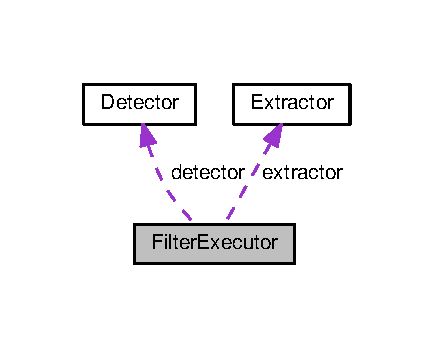
\includegraphics[width=208pt]{classFilterExecutor__coll__graph}
\end{center}
\end{figure}
\subsection*{Public Member Functions}
\begin{DoxyCompactItemize}
\item 
virtual \hyperlink{classFilterExecutor_a6dd36c64637e2747f1d997d4de5a121c}{$\sim$\+Filter\+Executor} ()
\begin{DoxyCompactList}\small\item\em Construct a new Filter Executor object. \end{DoxyCompactList}\item 
cv\+::\+Mat \hyperlink{classFilterExecutor_a06f4223dc3e15501aacc42b1f5bd026d}{filter} (const cv\+::\+Mat \&original, const \hyperlink{structSpecification}{Specification} \&specification)
\begin{DoxyCompactList}\small\item\em function that calls the necessary extraction -\/and detection function(s) to run a filter \end{DoxyCompactList}\item 
bool \hyperlink{classFilterExecutor_ab6054cdefd0e09ff04f2dd95489b1bea}{is\+Object} (const supported\+Shape \&shape, const std\+::vector$<$ std\+::vector$<$ cv\+::\+Point $>$$>$ \&contours, int index, \hyperlink{structFilterDetails}{Filter\+Details} \&filter\+Details) const 
\begin{DoxyCompactList}\small\item\em function that verifies if a set of contours is a specific function \end{DoxyCompactList}\item 
void \hyperlink{classFilterExecutor_a778b1fd0181990176842e5b107c0a76d}{set\+Display\+Mode} (const Display\+Mode \&a\+Display\+Mode)
\begin{DoxyCompactList}\small\item\em Set the Display Mode object. \end{DoxyCompactList}\end{DoxyCompactItemize}
\subsection*{Public Attributes}
\begin{DoxyCompactItemize}
\item 
\hyperlink{classExtractor}{Extractor} \hyperlink{classFilterExecutor_a4ab5f958ae995540afef4de2fc968d5d}{extractor}
\item 
\hyperlink{classDetector}{Detector} \hyperlink{classFilterExecutor_a5e2392a802b3aab62e95e5a7a7a066ae}{detector}
\end{DoxyCompactItemize}


\subsection{Detailed Description}
the filter executor combines the provided functionality by the detection and extraction classes. It will make sure every image is filtered properly and only the shape requested in a specification is marked. When finished it will make sure the result of a specification is showed to the user. 

\subsection{Constructor \& Destructor Documentation}
\index{Filter\+Executor@{Filter\+Executor}!````~Filter\+Executor@{$\sim$\+Filter\+Executor}}
\index{````~Filter\+Executor@{$\sim$\+Filter\+Executor}!Filter\+Executor@{Filter\+Executor}}
\subsubsection[{\texorpdfstring{$\sim$\+Filter\+Executor()}{~FilterExecutor()}}]{\setlength{\rightskip}{0pt plus 5cm}Filter\+Executor\+::$\sim$\+Filter\+Executor (
\begin{DoxyParamCaption}
{}
\end{DoxyParamCaption}
)\hspace{0.3cm}{\ttfamily [virtual]}}\hypertarget{classFilterExecutor_a6dd36c64637e2747f1d997d4de5a121c}{}\label{classFilterExecutor_a6dd36c64637e2747f1d997d4de5a121c}


Construct a new Filter Executor object. 

Destroy the Filter Executor object 

\subsection{Member Function Documentation}
\index{Filter\+Executor@{Filter\+Executor}!filter@{filter}}
\index{filter@{filter}!Filter\+Executor@{Filter\+Executor}}
\subsubsection[{\texorpdfstring{filter(const cv\+::\+Mat \&original, const Specification \&specification)}{filter(const cv::Mat &original, const Specification &specification)}}]{\setlength{\rightskip}{0pt plus 5cm}cv\+::\+Mat Filter\+Executor\+::filter (
\begin{DoxyParamCaption}
\item[{const cv\+::\+Mat \&}]{original, }
\item[{const {\bf Specification} \&}]{specification}
\end{DoxyParamCaption}
)}\hypertarget{classFilterExecutor_a06f4223dc3e15501aacc42b1f5bd026d}{}\label{classFilterExecutor_a06f4223dc3e15501aacc42b1f5bd026d}


function that calls the necessary extraction -\/and detection function(s) to run a filter 


\begin{DoxyParams}{Parameters}
{\em original} & the original frame where the filter has to be executed upon \\
\hline
{\em specification} & the specification contains information about the filter request \\
\hline
\end{DoxyParams}
\begin{DoxyReturn}{Returns}
cv\+::\+Mat the original image where the filter has run upon 
\end{DoxyReturn}
\index{Filter\+Executor@{Filter\+Executor}!is\+Object@{is\+Object}}
\index{is\+Object@{is\+Object}!Filter\+Executor@{Filter\+Executor}}
\subsubsection[{\texorpdfstring{is\+Object(const supported\+Shape \&shape, const std\+::vector$<$ std\+::vector$<$ cv\+::\+Point $>$$>$ \&contours, int index, Filter\+Details \&filter\+Details) const }{isObject(const supportedShape &shape, const std::vector< std::vector< cv::Point >> &contours, int index, FilterDetails &filterDetails) const }}]{\setlength{\rightskip}{0pt plus 5cm}bool Filter\+Executor\+::is\+Object (
\begin{DoxyParamCaption}
\item[{const supported\+Shape \&}]{shape, }
\item[{const std\+::vector$<$ std\+::vector$<$ cv\+::\+Point $>$$>$ \&}]{contours, }
\item[{int}]{index, }
\item[{{\bf Filter\+Details} \&}]{filter\+Details}
\end{DoxyParamCaption}
) const}\hypertarget{classFilterExecutor_ab6054cdefd0e09ff04f2dd95489b1bea}{}\label{classFilterExecutor_ab6054cdefd0e09ff04f2dd95489b1bea}


function that verifies if a set of contours is a specific function 


\begin{DoxyParams}{Parameters}
{\em shape} & the shape to be detected \\
\hline
{\em contours} & the detected set of contours \\
\hline
{\em index} & the position in the contours vector that indicates the current contour to be handled \\
\hline
{\em filter\+Details} & instance of struct \hyperlink{structFilterDetails}{Filter\+Details} that contain the result of the filter process \\
\hline
\end{DoxyParams}
\begin{DoxyReturn}{Returns}
true if the contours matched the shape to be detected 

false if the contours didn\textquotesingle{}t match the shape to be detected 
\end{DoxyReturn}
\index{Filter\+Executor@{Filter\+Executor}!set\+Display\+Mode@{set\+Display\+Mode}}
\index{set\+Display\+Mode@{set\+Display\+Mode}!Filter\+Executor@{Filter\+Executor}}
\subsubsection[{\texorpdfstring{set\+Display\+Mode(const Display\+Mode \&a\+Display\+Mode)}{setDisplayMode(const DisplayMode &aDisplayMode)}}]{\setlength{\rightskip}{0pt plus 5cm}void Filter\+Executor\+::set\+Display\+Mode (
\begin{DoxyParamCaption}
\item[{const Display\+Mode \&}]{a\+Display\+Mode}
\end{DoxyParamCaption}
)}\hypertarget{classFilterExecutor_a778b1fd0181990176842e5b107c0a76d}{}\label{classFilterExecutor_a778b1fd0181990176842e5b107c0a76d}


Set the Display Mode object. 


\begin{DoxyParams}{Parameters}
{\em a\+Display\+Mode} & the displaymode to be set \\
\hline
\end{DoxyParams}


\subsection{Member Data Documentation}
\index{Filter\+Executor@{Filter\+Executor}!detector@{detector}}
\index{detector@{detector}!Filter\+Executor@{Filter\+Executor}}
\subsubsection[{\texorpdfstring{detector}{detector}}]{\setlength{\rightskip}{0pt plus 5cm}{\bf Detector} Filter\+Executor\+::detector}\hypertarget{classFilterExecutor_a5e2392a802b3aab62e95e5a7a7a066ae}{}\label{classFilterExecutor_a5e2392a802b3aab62e95e5a7a7a066ae}
Detection instance detects certain objects after image extraction \index{Filter\+Executor@{Filter\+Executor}!extractor@{extractor}}
\index{extractor@{extractor}!Filter\+Executor@{Filter\+Executor}}
\subsubsection[{\texorpdfstring{extractor}{extractor}}]{\setlength{\rightskip}{0pt plus 5cm}{\bf Extractor} Filter\+Executor\+::extractor}\hypertarget{classFilterExecutor_a4ab5f958ae995540afef4de2fc968d5d}{}\label{classFilterExecutor_a4ab5f958ae995540afef4de2fc968d5d}
Extration instance extracs an image based on a color specified in a specification 

The documentation for this class was generated from the following files\+:\begin{DoxyCompactItemize}
\item 
src/Filter\+Executor.\+hpp\item 
src/Filter\+Executor.\+cpp\end{DoxyCompactItemize}

\hypertarget{classInteractiveApplication}{}\section{Interactive\+Application Class Reference}
\label{classInteractiveApplication}\index{Interactive\+Application@{Interactive\+Application}}


Instance of an application. The interactive application starts the interactive mode in the \hyperlink{classInteractiveApplication_ae77593fe90fa4fae53dc8ca84ba1a239}{run()} function that stays active until the user specifies the \textquotesingle{}exit\textquotesingle{} command on the console. The application will display the result for a specification until a new specification is given.  




{\ttfamily \#include $<$Interactive\+Application.\+hpp$>$}



Inheritance diagram for Interactive\+Application\+:\nopagebreak
\begin{figure}[H]
\begin{center}
\leavevmode
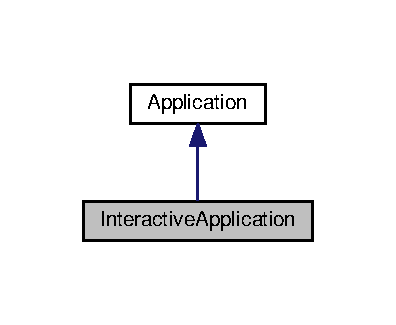
\includegraphics[width=190pt]{classInteractiveApplication__inherit__graph}
\end{center}
\end{figure}


Collaboration diagram for Interactive\+Application\+:\nopagebreak
\begin{figure}[H]
\begin{center}
\leavevmode
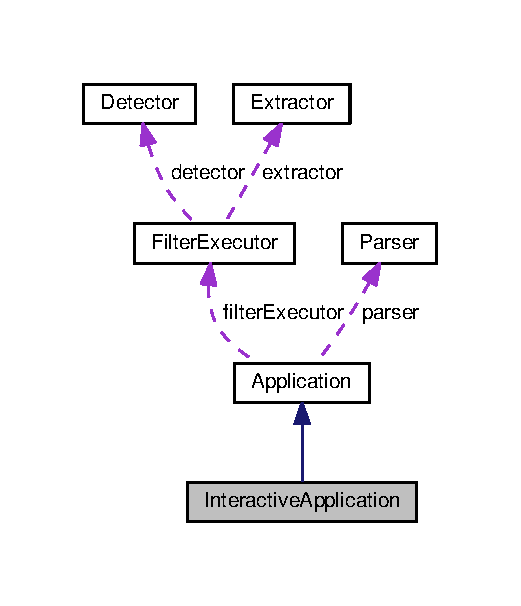
\includegraphics[width=250pt]{classInteractiveApplication__coll__graph}
\end{center}
\end{figure}
\subsection*{Public Member Functions}
\begin{DoxyCompactItemize}
\item 
\hyperlink{classInteractiveApplication_a400252d4a0553cc7fb85106106341fe9}{Interactive\+Application} (const std\+::string \&a\+Name)\hypertarget{classInteractiveApplication_a400252d4a0553cc7fb85106106341fe9}{}\label{classInteractiveApplication_a400252d4a0553cc7fb85106106341fe9}

\begin{DoxyCompactList}\small\item\em constructor of the interactive application \end{DoxyCompactList}\item 
virtual \hyperlink{classInteractiveApplication_adebc1def706d551144ab3f40511f85eb}{$\sim$\+Interactive\+Application} ()\hypertarget{classInteractiveApplication_adebc1def706d551144ab3f40511f85eb}{}\label{classInteractiveApplication_adebc1def706d551144ab3f40511f85eb}

\begin{DoxyCompactList}\small\item\em destructor of the interactive application \end{DoxyCompactList}\item 
void \hyperlink{classInteractiveApplication_ae77593fe90fa4fae53dc8ca84ba1a239}{run} ()\hypertarget{classInteractiveApplication_ae77593fe90fa4fae53dc8ca84ba1a239}{}\label{classInteractiveApplication_ae77593fe90fa4fae53dc8ca84ba1a239}

\begin{DoxyCompactList}\small\item\em function that runs the application\+: overrides the pure virtual run -\/function in \hyperlink{Application_8hpp_source}{Application.\+hpp} \end{DoxyCompactList}\item 
void \hyperlink{classInteractiveApplication_a8fb03895eb606ec5b984b5f0d10aca53}{read\+New\+Specifications} ()\hypertarget{classInteractiveApplication_a8fb03895eb606ec5b984b5f0d10aca53}{}\label{classInteractiveApplication_a8fb03895eb606ec5b984b5f0d10aca53}

\begin{DoxyCompactList}\small\item\em function that reads and parses new specifications 
\begin{DoxyExceptions}{Exceptions}
{\em std\+::invalid\+\_\+argument} & if an invalid specification was entered by the user \\
\hline
\end{DoxyExceptions}
\end{DoxyCompactList}\end{DoxyCompactItemize}
\subsection*{Additional Inherited Members}


\subsection{Detailed Description}
Instance of an application. The interactive application starts the interactive mode in the \hyperlink{classInteractiveApplication_ae77593fe90fa4fae53dc8ca84ba1a239}{run()} function that stays active until the user specifies the \textquotesingle{}exit\textquotesingle{} command on the console. The application will display the result for a specification until a new specification is given. 

The documentation for this class was generated from the following files\+:\begin{DoxyCompactItemize}
\item 
src/Interactive\+Application.\+hpp\item 
src/Interactive\+Application.\+cpp\end{DoxyCompactItemize}

\hypertarget{classParser}{}\section{Parser Class Reference}
\label{classParser}\index{Parser@{Parser}}


the parser contains all functionality to parse batch files and specifications.  




{\ttfamily \#include $<$Parser.\+hpp$>$}

\subsection*{Public Member Functions}
\begin{DoxyCompactItemize}
\item 
\hyperlink{classParser_a12234f6cd36b61af4b50c94a179422c1}{Parser} ()\hypertarget{classParser_a12234f6cd36b61af4b50c94a179422c1}{}\label{classParser_a12234f6cd36b61af4b50c94a179422c1}

\begin{DoxyCompactList}\small\item\em default constructor of the specification parser \end{DoxyCompactList}\item 
virtual \hyperlink{classParser_a3e658b5917a93a3ef648050d060e3a93}{$\sim$\+Parser} ()\hypertarget{classParser_a3e658b5917a93a3ef648050d060e3a93}{}\label{classParser_a3e658b5917a93a3ef648050d060e3a93}

\begin{DoxyCompactList}\small\item\em destructor of the specification parser \end{DoxyCompactList}\item 
bool \hyperlink{classParser_a8af5f2b3cbe50b7b4ad41e0a54dd70f5}{try\+Parse\+Specification\+From\+Str} (const std\+::string \&str, \hyperlink{structSpecification}{Specification} \&specification)
\begin{DoxyCompactList}\small\item\em function that tries to create a specification object of a string \end{DoxyCompactList}\item 
bool \hyperlink{classParser_a5c5356810a3861d9fe50353fbd00040e}{try\+Parse\+Batch\+Config} (const std\+::string \&batch\+Config\+Path, std\+::vector$<$ \hyperlink{structSpecification}{Specification} $>$ \&specifications)
\begin{DoxyCompactList}\small\item\em function that tries to convert a batchfile into a list of specifications \end{DoxyCompactList}\item 
supported\+Color \hyperlink{classParser_abfb3329a63d465462db4778609abd18a}{color\+From\+Str} (const std\+::string \&str) const 
\begin{DoxyCompactList}\small\item\em function that converts a string into a supported color (read \hyperlink{SpecificationConfig_8hpp_source}{src/\+Specification\+Config.\+hpp} for the supported colors) \end{DoxyCompactList}\item 
supported\+Shape \hyperlink{classParser_a2530730579b210a6d64154404b670eea}{shape\+From\+Str} (const std\+::string \&str) const 
\begin{DoxyCompactList}\small\item\em function that converts a string into a supported shape (read \hyperlink{SpecificationConfig_8hpp_source}{src/\+Specification\+Config.\+hpp} for the supported shapes) \end{DoxyCompactList}\item 
const std\+::string \hyperlink{classParser_a8453d650d2ac054b3ca603eca69802db}{str\+From\+Color} (const supported\+Color \&color)
\begin{DoxyCompactList}\small\item\em function that converts a color into its string representation \end{DoxyCompactList}\item 
const std\+::string \hyperlink{classParser_a5938f4f0fb88e6a5a4fdc1e795920bb3}{str\+From\+Shape} (const supported\+Shape \&shape)
\begin{DoxyCompactList}\small\item\em function that converts a shape into its string representation \end{DoxyCompactList}\end{DoxyCompactItemize}


\subsection{Detailed Description}
the parser contains all functionality to parse batch files and specifications. 

\subsection{Member Function Documentation}
\index{Parser@{Parser}!color\+From\+Str@{color\+From\+Str}}
\index{color\+From\+Str@{color\+From\+Str}!Parser@{Parser}}
\subsubsection[{\texorpdfstring{color\+From\+Str(const std\+::string \&str) const }{colorFromStr(const std::string &str) const }}]{\setlength{\rightskip}{0pt plus 5cm}supported\+Color Parser\+::color\+From\+Str (
\begin{DoxyParamCaption}
\item[{const std\+::string \&}]{str}
\end{DoxyParamCaption}
) const}\hypertarget{classParser_abfb3329a63d465462db4778609abd18a}{}\label{classParser_abfb3329a63d465462db4778609abd18a}


function that converts a string into a supported color (read \hyperlink{SpecificationConfig_8hpp_source}{src/\+Specification\+Config.\+hpp} for the supported colors) 


\begin{DoxyParams}{Parameters}
{\em str} & the string to be converted \\
\hline
\end{DoxyParams}
\begin{DoxyReturn}{Returns}
const supported\+Color the supported color instance 
\end{DoxyReturn}

\begin{DoxyExceptions}{Exceptions}
{\em if} & an invalid string was given \\
\hline
\end{DoxyExceptions}
\index{Parser@{Parser}!shape\+From\+Str@{shape\+From\+Str}}
\index{shape\+From\+Str@{shape\+From\+Str}!Parser@{Parser}}
\subsubsection[{\texorpdfstring{shape\+From\+Str(const std\+::string \&str) const }{shapeFromStr(const std::string &str) const }}]{\setlength{\rightskip}{0pt plus 5cm}supported\+Shape Parser\+::shape\+From\+Str (
\begin{DoxyParamCaption}
\item[{const std\+::string \&}]{str}
\end{DoxyParamCaption}
) const}\hypertarget{classParser_a2530730579b210a6d64154404b670eea}{}\label{classParser_a2530730579b210a6d64154404b670eea}


function that converts a string into a supported shape (read \hyperlink{SpecificationConfig_8hpp_source}{src/\+Specification\+Config.\+hpp} for the supported shapes) 


\begin{DoxyParams}{Parameters}
{\em str} & the string to be converted \\
\hline
\end{DoxyParams}
\begin{DoxyReturn}{Returns}
const supported\+Shape the supported shape instance 
\end{DoxyReturn}

\begin{DoxyExceptions}{Exceptions}
{\em if} & an invalid string was given \\
\hline
\end{DoxyExceptions}
\index{Parser@{Parser}!str\+From\+Color@{str\+From\+Color}}
\index{str\+From\+Color@{str\+From\+Color}!Parser@{Parser}}
\subsubsection[{\texorpdfstring{str\+From\+Color(const supported\+Color \&color)}{strFromColor(const supportedColor &color)}}]{\setlength{\rightskip}{0pt plus 5cm}const std\+::string Parser\+::str\+From\+Color (
\begin{DoxyParamCaption}
\item[{const supported\+Color \&}]{color}
\end{DoxyParamCaption}
)}\hypertarget{classParser_a8453d650d2ac054b3ca603eca69802db}{}\label{classParser_a8453d650d2ac054b3ca603eca69802db}


function that converts a color into its string representation 


\begin{DoxyParams}{Parameters}
{\em color} & the color instance to be converted \\
\hline
\end{DoxyParams}
\begin{DoxyReturn}{Returns}
const std\+::string the string representation of the color 
\end{DoxyReturn}
\index{Parser@{Parser}!str\+From\+Shape@{str\+From\+Shape}}
\index{str\+From\+Shape@{str\+From\+Shape}!Parser@{Parser}}
\subsubsection[{\texorpdfstring{str\+From\+Shape(const supported\+Shape \&shape)}{strFromShape(const supportedShape &shape)}}]{\setlength{\rightskip}{0pt plus 5cm}const std\+::string Parser\+::str\+From\+Shape (
\begin{DoxyParamCaption}
\item[{const supported\+Shape \&}]{shape}
\end{DoxyParamCaption}
)}\hypertarget{classParser_a5938f4f0fb88e6a5a4fdc1e795920bb3}{}\label{classParser_a5938f4f0fb88e6a5a4fdc1e795920bb3}


function that converts a shape into its string representation 


\begin{DoxyParams}{Parameters}
{\em shape} & the shape instance to be converted \\
\hline
\end{DoxyParams}
\begin{DoxyReturn}{Returns}
const std\+::string the string representation of the shape 
\end{DoxyReturn}
\index{Parser@{Parser}!try\+Parse\+Batch\+Config@{try\+Parse\+Batch\+Config}}
\index{try\+Parse\+Batch\+Config@{try\+Parse\+Batch\+Config}!Parser@{Parser}}
\subsubsection[{\texorpdfstring{try\+Parse\+Batch\+Config(const std\+::string \&batch\+Config\+Path, std\+::vector$<$ Specification $>$ \&specifications)}{tryParseBatchConfig(const std::string &batchConfigPath, std::vector< Specification > &specifications)}}]{\setlength{\rightskip}{0pt plus 5cm}bool Parser\+::try\+Parse\+Batch\+Config (
\begin{DoxyParamCaption}
\item[{const std\+::string \&}]{batch\+Config\+Path, }
\item[{std\+::vector$<$ {\bf Specification} $>$ \&}]{specifications}
\end{DoxyParamCaption}
)}\hypertarget{classParser_a5c5356810a3861d9fe50353fbd00040e}{}\label{classParser_a5c5356810a3861d9fe50353fbd00040e}


function that tries to convert a batchfile into a list of specifications 


\begin{DoxyParams}{Parameters}
{\em batch\+Config\+Path} & the path to the batchfile that contains the specifications \\
\hline
{\em specifications} & the list where the converted specifications will be stored in \\
\hline
\end{DoxyParams}
\begin{DoxyReturn}{Returns}
true if the convertion was successfull 

false if the batch file couldnt be converted 
\end{DoxyReturn}

\begin{DoxyExceptions}{Exceptions}
{\em if} & the batchfile contains syntax errors \\
\hline
\end{DoxyExceptions}
\index{Parser@{Parser}!try\+Parse\+Specification\+From\+Str@{try\+Parse\+Specification\+From\+Str}}
\index{try\+Parse\+Specification\+From\+Str@{try\+Parse\+Specification\+From\+Str}!Parser@{Parser}}
\subsubsection[{\texorpdfstring{try\+Parse\+Specification\+From\+Str(const std\+::string \&str, Specification \&specification)}{tryParseSpecificationFromStr(const std::string &str, Specification &specification)}}]{\setlength{\rightskip}{0pt plus 5cm}bool Parser\+::try\+Parse\+Specification\+From\+Str (
\begin{DoxyParamCaption}
\item[{const std\+::string \&}]{str, }
\item[{{\bf Specification} \&}]{specification}
\end{DoxyParamCaption}
)}\hypertarget{classParser_a8af5f2b3cbe50b7b4ad41e0a54dd70f5}{}\label{classParser_a8af5f2b3cbe50b7b4ad41e0a54dd70f5}


function that tries to create a specification object of a string 


\begin{DoxyParams}{Parameters}
{\em str} & the string to be converted to a specification \\
\hline
{\em specification} & reference to the specification where the string data will be stored in \\
\hline
\end{DoxyParams}
\begin{DoxyReturn}{Returns}
true if the string was successfully converted 

false if the string wasnt successfully converted 
\end{DoxyReturn}

\begin{DoxyExceptions}{Exceptions}
{\em if} & the string could not be converted \\
\hline
\end{DoxyExceptions}


The documentation for this class was generated from the following files\+:\begin{DoxyCompactItemize}
\item 
src/Parser.\+hpp\item 
src/Parser.\+cpp\end{DoxyCompactItemize}

\hypertarget{structSpecification}{}\section{Specification Struct Reference}
\label{structSpecification}\index{Specification@{Specification}}


filtering process is based on a specification. This struct describes the attributes a specification has.  




{\ttfamily \#include $<$Specification.\+hpp$>$}

\subsection*{Public Member Functions}
\begin{DoxyCompactItemize}
\item 
\hyperlink{structSpecification_a1da67067067a6876811fe1af3dc09ef0}{Specification} ()\hypertarget{structSpecification_a1da67067067a6876811fe1af3dc09ef0}{}\label{structSpecification_a1da67067067a6876811fe1af3dc09ef0}

\begin{DoxyCompactList}\small\item\em default constructor of a specification \end{DoxyCompactList}\item 
\hyperlink{structSpecification_aa08664e5866421d776266b69c90138cb}{Specification} (const \hyperlink{structSpecification}{Specification} \&rhs)
\begin{DoxyCompactList}\small\item\em Construct a new \hyperlink{structSpecification}{Specification} object (copyconstructor) \end{DoxyCompactList}\item 
\hyperlink{structSpecification_a9e5dea83bffde839da128d4551a6a691}{$\sim$\+Specification} ()\hypertarget{structSpecification_a9e5dea83bffde839da128d4551a6a691}{}\label{structSpecification_a9e5dea83bffde839da128d4551a6a691}

\begin{DoxyCompactList}\small\item\em destructor of a specification \end{DoxyCompactList}\item 
\hyperlink{structSpecification}{Specification} \& \hyperlink{structSpecification_a63c2bfcc3247194eaaf72126de1888aa}{operator=} (const \hyperlink{structSpecification}{Specification} \&rhs)
\begin{DoxyCompactList}\small\item\em Assignment operator for a specification. \end{DoxyCompactList}\end{DoxyCompactItemize}
\subsection*{Public Attributes}
\begin{DoxyCompactItemize}
\item 
supported\+Shape \hyperlink{structSpecification_a07d43e0225d3d091376ff907493d9f5e}{shape}
\item 
supported\+Color \hyperlink{structSpecification_a84179e823020d11ac7fa9e063d5f0b53}{color}
\item 
bool \hyperlink{structSpecification_ace792a91a5cee16442844dc7b4099974}{exit} = false
\end{DoxyCompactItemize}


\subsection{Detailed Description}
filtering process is based on a specification. This struct describes the attributes a specification has. 

\subsection{Constructor \& Destructor Documentation}
\index{Specification@{Specification}!Specification@{Specification}}
\index{Specification@{Specification}!Specification@{Specification}}
\subsubsection[{\texorpdfstring{Specification(const Specification \&rhs)}{Specification(const Specification &rhs)}}]{\setlength{\rightskip}{0pt plus 5cm}Specification\+::\+Specification (
\begin{DoxyParamCaption}
\item[{const {\bf Specification} \&}]{rhs}
\end{DoxyParamCaption}
)}\hypertarget{structSpecification_aa08664e5866421d776266b69c90138cb}{}\label{structSpecification_aa08664e5866421d776266b69c90138cb}


Construct a new \hyperlink{structSpecification}{Specification} object (copyconstructor) 


\begin{DoxyParams}{Parameters}
{\em rhs} & the object to be copied \\
\hline
\end{DoxyParams}


\subsection{Member Function Documentation}
\index{Specification@{Specification}!operator=@{operator=}}
\index{operator=@{operator=}!Specification@{Specification}}
\subsubsection[{\texorpdfstring{operator=(const Specification \&rhs)}{operator=(const Specification &rhs)}}]{\setlength{\rightskip}{0pt plus 5cm}{\bf Specification} \& Specification\+::operator= (
\begin{DoxyParamCaption}
\item[{const {\bf Specification} \&}]{rhs}
\end{DoxyParamCaption}
)}\hypertarget{structSpecification_a63c2bfcc3247194eaaf72126de1888aa}{}\label{structSpecification_a63c2bfcc3247194eaaf72126de1888aa}


Assignment operator for a specification. 


\begin{DoxyParams}{Parameters}
{\em rhs} & contains the values to be assigned \\
\hline
\end{DoxyParams}
\begin{DoxyReturn}{Returns}
\hyperlink{structSpecification}{Specification}\& the specification instance with the set values 
\end{DoxyReturn}


\subsection{Member Data Documentation}
\index{Specification@{Specification}!color@{color}}
\index{color@{color}!Specification@{Specification}}
\subsubsection[{\texorpdfstring{color}{color}}]{\setlength{\rightskip}{0pt plus 5cm}supported\+Color Specification\+::color}\hypertarget{structSpecification_a84179e823020d11ac7fa9e063d5f0b53}{}\label{structSpecification_a84179e823020d11ac7fa9e063d5f0b53}
The color that the shape is supposed to have according to this specification instance \index{Specification@{Specification}!exit@{exit}}
\index{exit@{exit}!Specification@{Specification}}
\subsubsection[{\texorpdfstring{exit}{exit}}]{\setlength{\rightskip}{0pt plus 5cm}bool Specification\+::exit = false}\hypertarget{structSpecification_ace792a91a5cee16442844dc7b4099974}{}\label{structSpecification_ace792a91a5cee16442844dc7b4099974}
Contains a bool value, true if the specification tells the interactive mode to shutdown \index{Specification@{Specification}!shape@{shape}}
\index{shape@{shape}!Specification@{Specification}}
\subsubsection[{\texorpdfstring{shape}{shape}}]{\setlength{\rightskip}{0pt plus 5cm}supported\+Shape Specification\+::shape}\hypertarget{structSpecification_a07d43e0225d3d091376ff907493d9f5e}{}\label{structSpecification_a07d43e0225d3d091376ff907493d9f5e}
The shape to be detected according to this specification instance 

The documentation for this struct was generated from the following files\+:\begin{DoxyCompactItemize}
\item 
src/Specification.\+hpp\item 
src/Specification.\+cpp\end{DoxyCompactItemize}

%--- End generated contents ---

% Index
\backmatter
\newpage
\phantomsection
\clearemptydoublepage
\addcontentsline{toc}{chapter}{Index}
\printindex

\end{document}
